\chapter{Case study: the iTrust SWaT System}
\label{casestudy}

%\linenumbers
\lettrine[lines=2]{H}{aving} introduced the innovative framework and highlighted its potential in the preceding chapter, we now turn our attention to the case study where we will apply this framework. As previously mentioned in Chapter \ref{chap:proposal} and demonstrated through various examples in the same chapter, our focus will be on the \textbf{iTrust SWaT system} \cite{swat_home}, developed by the iTrust -- Center for Research in Cyber Security of University of Singapore for Technology and Design \cite{itrust_site}. The acronym SWaT represents \textit{\textbf{S}ecure \textbf{Wa}ter \textbf{T}reatment}.

\bigskip
The iTrust SWaT system is a testbed that replicates on a small scale a real water treatment plant arises to support research in the area of cyber security of industrial control systems and has been operational since March 2015: it is still being used by students at the University of Singapore for educational and training purposes and is available to organizations to train their operators on cyber physical incidents.

\section{Architecture}
\label{sec:5_swat_architecture}
In contrast to the virtualized testbed discussed in Section \ref{subsec:3_testbed} by Ceccato et al., the iTrust SWaT system is composed entirely of physical hardware components. It encompasses various elements, starting from field devices and extending to PLCs, HMI, SCADA workstations, and the SCADA server (also referred to as the \textit{historian}). The historian is responsible for recording data from field devices for further analysis. In the upcoming sections, we will delve deeper into the architecture of the physical process and the communication network.

\subsection{Physical Process} 
\label{subsec:5_swat_physical_architecture}
The physical process of the SWaT consists of six stages, denoted P1 through P6 \cite{swat_tecnical_pdf}\cite{swat_tippenhauer}. These stages are:

\begin{enumerate}
	\item[P1.] \textbf{taking in raw water:} feeds unfiltered water into the system
	
	\item[P2.] \textbf{chemical dosing:} adds chemicals to water useful for initial pretreatment;
	
	\item[P3.] \textbf{Ultra Filtration (UF) system:} the water is filtered through a semi-permeable membrane (ultrafiltration membrane) using the liquid pressure, effectively capturing impurities and suspended solids, as well as removing bacteria, viruses, and other pathogens present in the water;
	
	\item[P4.] \textbf{dechlorination:} removes residual chlorine from disinfected water using ultraviolet lamps;
	
	\item[P5.] \textbf{Reverse Osmosis (RO):} performs further filtration of the water;
	
	\item[P6.] \textbf{backwash process:} cleans the membranes in UF using the water produced by RO.
	
\end{enumerate}

\noindent Figure \ref{fig:5_swat_architecture_1} \cite{swat_home} shows a graphical representation of the architecture and the six stages of the SWaT system.

\begin{figure}[ht]
	\centering
	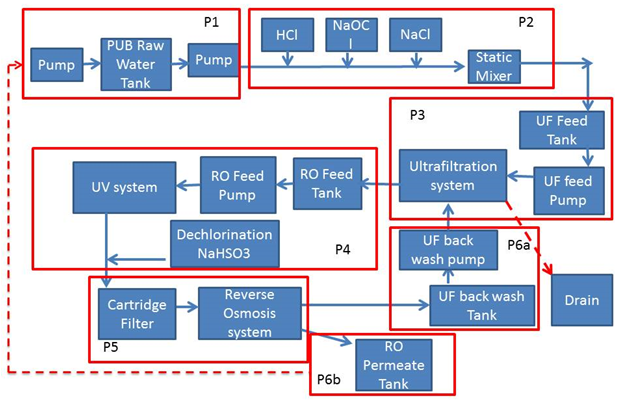
\includegraphics[scale=0.55]{chap5/testbed-3.png}
	\caption{SWaT architecture}
	\label{fig:5_swat_architecture_1}
\end{figure}

\bigskip
The SWaT system incorporates an array of sensors that play a crucial role in monitoring the system's operations and ensuring their safety. These sensors are responsible for continuously collecting data and providing interesting insights into the functioning of the system \cite{swat_tecnical_pdf}. These sensors are:

\begin{itemize}
	\item Level Indication Transmitter (measured in mm);
	\item Flow Indication Transmitter (m3/hr);
	\item Analyser Indicator Transmitter;
	\begin{itemize}
		\item[o] Conductivity (µS/cm);
		\item[o] pH;
		\item[o] Oxidation Reduction Potential (mV);
	\end{itemize}
	\item Differential Pressure Indicator Transmitter (kPa);
	\item Pressure Indicator Transmitter (kPa);
\end{itemize}

Sensors and actuators associated with each PLC are shown in Figure \ref{fig:5_swat_sensors_plc} \cite{swat_tecnical_pdf}.
Sensors and actuators are mapped into tags by the communication protocol used (see \ref{subsec:5_swat_network_architecture}): a tag can be addressed via string descriptor defined by the system designer (e.g. MV101, to indicate motorized valve number 1 at stage 1) or by referring directly to the analog/digital pins of the PLC I/O unit \cite{swat_tippenhauer}.

\begin{figure}[ht]
	\centering
	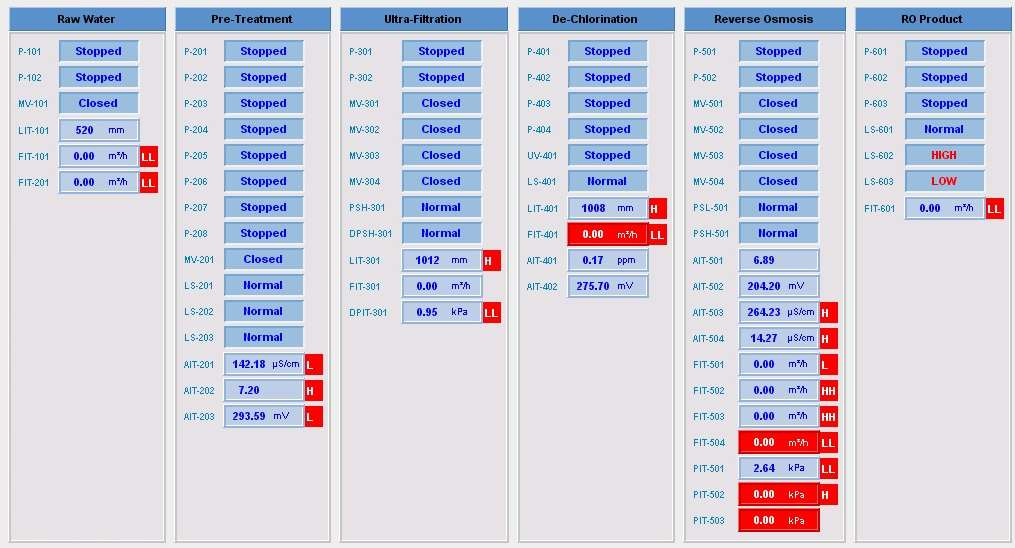
\includegraphics[scale=0.50]{chap5/plc-devices.jpg}
	\caption{Sensors and actuators associated with each PLC}
	\label{fig:5_swat_sensors_plc}
\end{figure}

\subsection{Control and Communication Network}
\label{subsec:5_swat_network_architecture}
The SWaT system's network architecture follows the principles of layering and zoning, which enable segmentation and control of traffic within the network.
\newline \newline
Five layers are present starting from the highest to the lowest: 

\begin{itemize}
	\item \textbf{Layer 3.5} -- Demilitarized Zone (DMZ);
	\item \textbf{Layer 3} -- Operation Management (Historian);
	\item \textbf{Layer 2} -- Supervisory Control (Touch Panel, Engineering Workstation, HMI Control Clients);
	\item \textbf{Layer 1} -- Plant Control Network (PLCs) (Star Network);
	\item \textbf{Layer 0} -- Process (Actuator/Sensors and Input/output modules) (Ring Network).
\end{itemize}

PLCs at Layer 1 communicate with their respective sensors and actuators at Layer 0 through a conventional ring network topology based on EtherNet/IP, to ensure that the system can tolerate the loss of a single link without any adverse impact on data or control functionality.

PLCs between the different process stages at Layer 1 communicate with each other through a star network topology using the CIP protocol on EtherNet/IP, previously discussed in Section \ref{subsubsec:2_cip}.

\bigskip
Regarding zoning, the SWaT system is divided into three zones, each containing one or more layers. These zones are, in descending order of security level: 

\begin{itemize}
	\item \textbf{Plant Control Network}, or \textbf{Control System:} includes layers from 0 to 2;
	\item \textbf{DMZ:} includes Layer 3.5;
	\item \textbf{Plant Network:} includes Layer 3;
\end{itemize}

Figure \ref{fig:5_swat_network_arch} \cite{swat_home} provides a clearer visualization of the zoning and layer division within the network architecture of the SWaT system. This diagram highlights the distinct zones and their corresponding layers, offering a comprehensive overview of the system's network structure.

\bigskip
A specific IP address is associated with each device: in Table \ref{table:5_swat_ip_addresses} we report the addresses for the PLCs, historian, and Touch Panel in the \textit{Plant Control Network} (PCN) zone:

\bigskip
{\small
\begin{longtable}[c]{p{0.30\textwidth} p{0.45\textwidth}}
	\hline
	\textbf{IP Address} & \textbf{Device} \\ [0.5ex] 
	\hline
	192.168.1.10 & PLC1 \\
	\hline 
	192.168.1.20 & PLC2 \\
	\hline
	192.168.1.30 & PLC3 \\
	\hline
	192.168.1.40 & PLC4 \\
	\hline
	192.168.1.50 & PLC5 \\
	\hline
	192.168.1.60 & PLC6 \\
	\hline
	192.168.1.100 & {Touch Panel (PCN)} \\
	\hline
	192.168.1.200 & Historian Server \\
	\hline
	192.168.1.201 & Engineering Workstation \\
	\hline
	
	\caption{Main IP addresses of the six PLCs and SCADA in the SWaT system}
	\label{table:5_swat_ip_addresses}
\end{longtable}
}

\begin{figure}[ht]
	\centering
	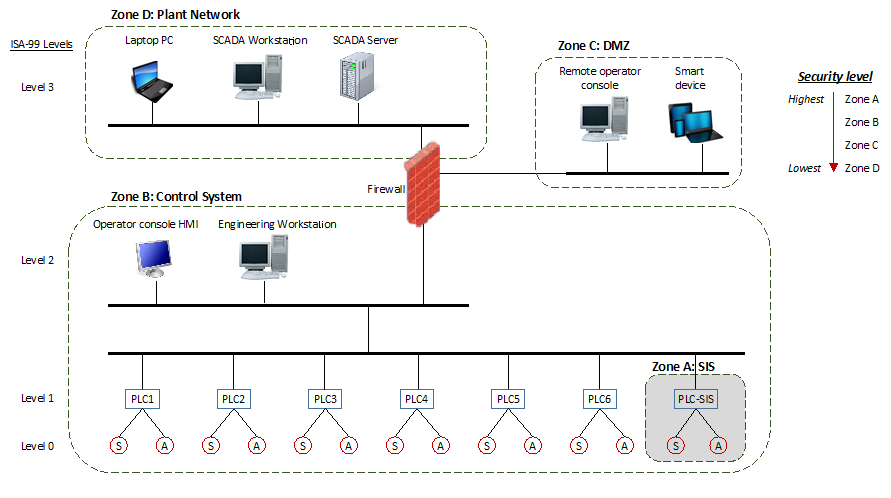
\includegraphics[scale=0.60]{chap5/testbed-4.png}
	\caption{SWaT network architecture and zoning}
	\label{fig:5_swat_network_arch}
\end{figure}

\section{Datasets}
\label{sec:5_swat_datasets}

To facilitate the study and testing of technologies related to cyber security in Industrial Control Systems and critical infrastructure, iTrust offers researchers worldwide the opportunity to access a range of datasets \cite{swat_datasets}. These datasets consist of a collection of data obtained from the SWaT system, encompassing information on both the physical processes and network communications. The data is organized into different years, and researchers can request access to these datasets for their analysis and experimentation purposes.

\bigskip
\paragraph{Physical Process Datasets}
The datasets containing information about the physical processes are provided in CSV format files. These files encompass data collected during different time intervals, which can vary from a few hours to entire days. The granularity of the data is typically at a one-second interval, although there may be some exceptions. The collected data primarily consists of timestamped sensor measurements and actuator status values for each PLC, describing the physical properties of the testbed in operational mode.

\paragraph{Network Communications Datasets}
Network communications are typically available in the form of \textit{Packet Capture} format (PCAP) files. These files contain captures of communication network traffic, allowing researchers to analyze and examine the network interactions. In some instances, CSV files are provided instead of PCAP files, featuring different characteristics for the collected data.

\subsection{Our Case Study: the 2015 Dataset}
\label{subsec:5_2015_datasets}
The dataset selected as a case study to apply the framework discussed in the previous chapter is specifically the dataset from the year 2015 \cite{swat_dataset2015}. The main reason for this choice is the unique characteristics found in the physical process dataset that are not present in datasets from subsequent years.

\paragraph{Physical Process Data}
\label{par:5_2015_physical_dataset}
The data collection process lasted 11 consecutive days, 24 hours per day. During the first 7 days, the system operated normally without any recorded attacks. However, attacks were observed during the remaining 4 days. The collected data reflects the impact of these attacks, leading to the creation of two separate CSV files: one containing the recorded data of SWaT during the system's regular operations, and the other containing data recorded during the days of the attacks. To ensure accurate information about the system, the dataset pertaining to the normal operations, which spans seven days, was chosen for analysis.

\bigskip
Data collection occurs at a frequency of one data point per second, with the assumption that significant attacks cannot occur within a shorter time frame. Additionally, the firmware of the PLCs remains unchanged throughout the data collection period.\newline
At the beginning of data gathering the tanks are empty and the system must be initialized in order to then reach full operation: it typically takes around five hours for all tanks to be fully filled and for the system to stabilize and reach the appropriate operational state (see Figure \ref{fig:5_swat_stabilization}).

\begin{figure}[ht]
	\centering
	\begin{subfigure}{0.48\textwidth}
		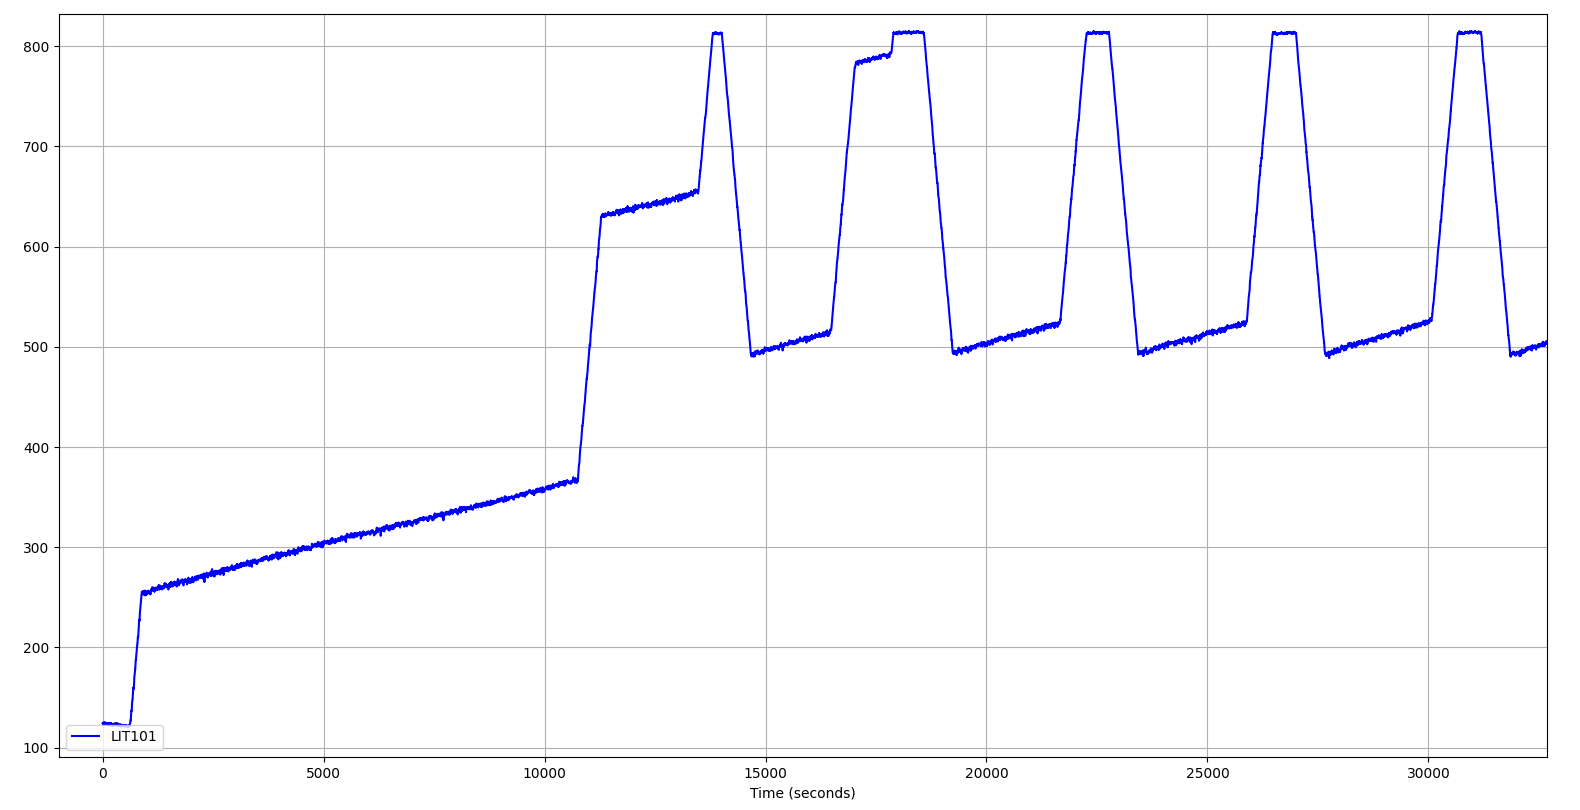
\includegraphics[width=\textwidth]{chap5/stabilizzazione_P1.png}
		\caption{Stabilization of \texttt{P1\_LIT101}}
		\label{subfig:5_stab_lit101}
	\end{subfigure}
	\hfill
	\begin{subfigure}{0.48\textwidth}
		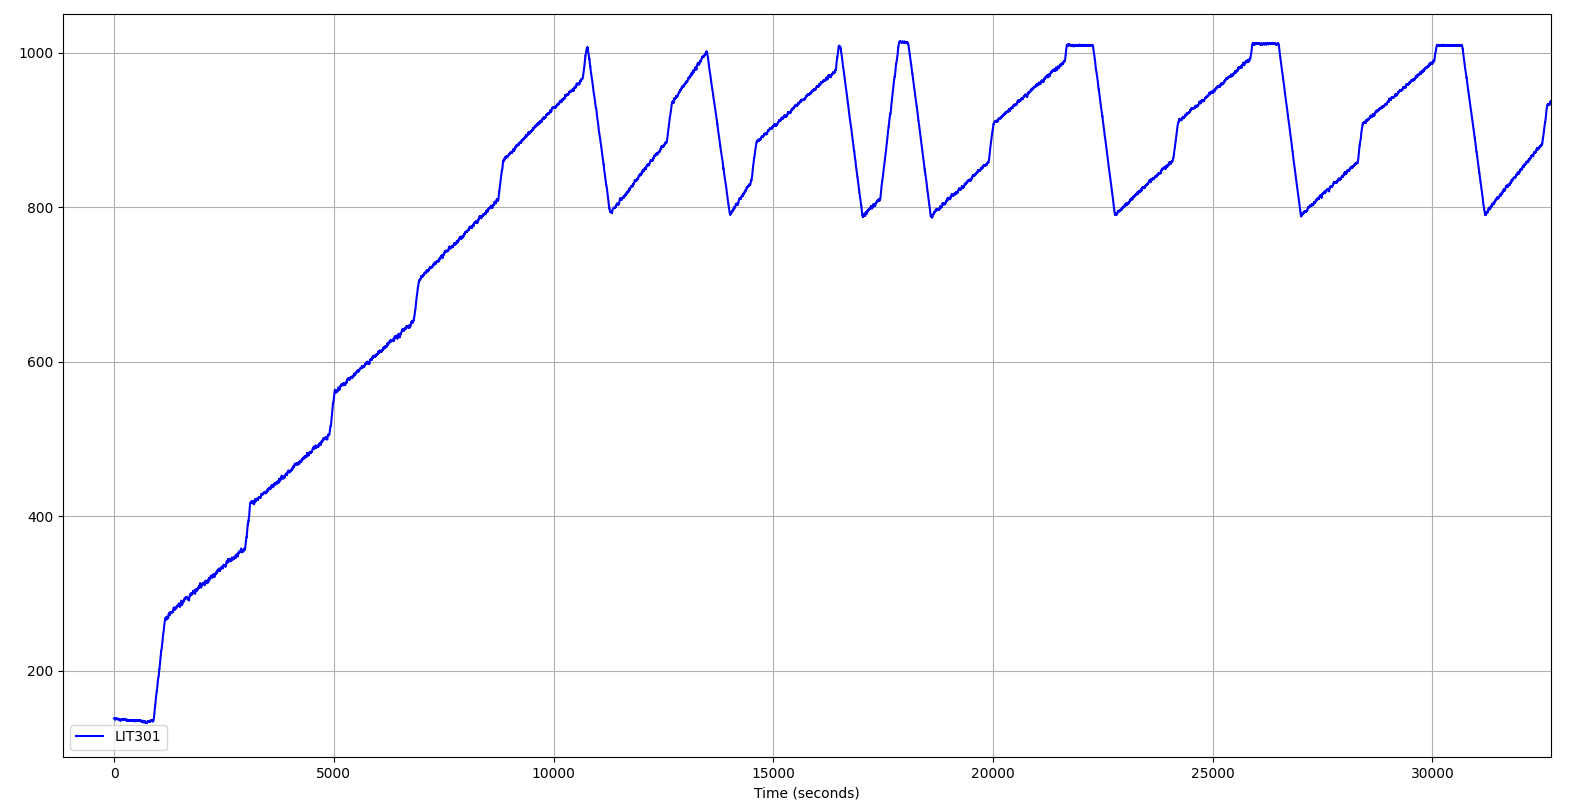
\includegraphics[width=\textwidth]{chap5/stabilizzazione_P3.png}
		\caption{Stabilization of \texttt{P3\_LIT301}}
		\label{subfig:5_stab_lit301}
	\end{subfigure}
	\begin{subfigure}{0.48\textwidth}
		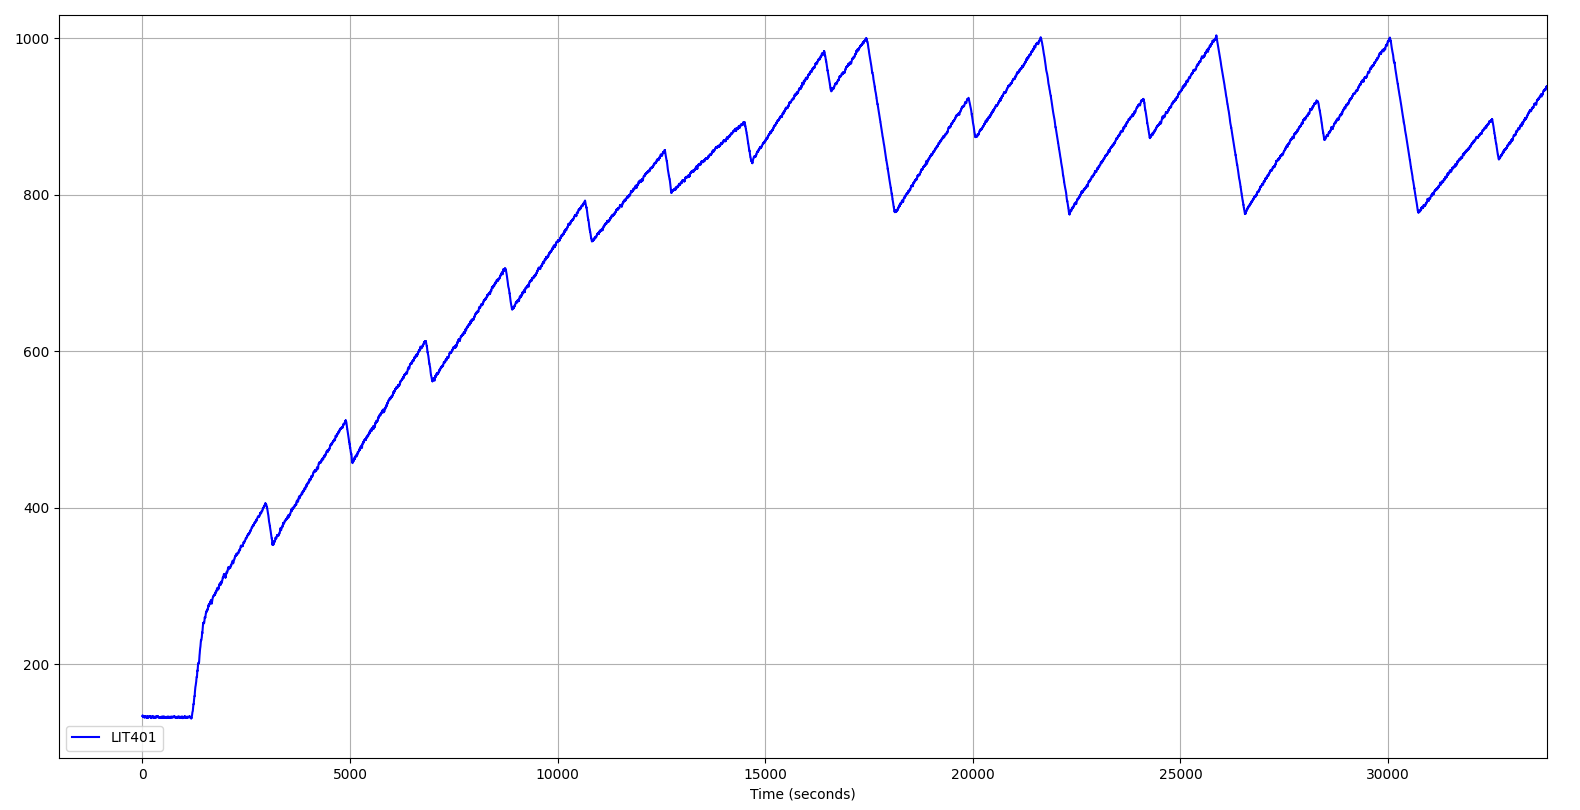
\includegraphics[width=\textwidth]{chap5/stabilizzazione_P4.png}
		\caption{Stabilization of \texttt{P4\_LIT401}}
		\label{subfig:5_stab_lit401}
	\end{subfigure}
	\caption{SWaT stabilization}
	\label{fig:5_swat_stabilization}
\end{figure}
In total, the dataset consists of thousands of lines collecting 51 attributes denoting the state of the system.

\paragraph{Network Traffic}
\label{par:5_2015_net_dataset}
The network traffic was collected using an appliance from a well-known network hardware manufacturer and was made available only in CSV format and not PCAP format. Table \ref{table:5_swat_network_traffic_data} shows some of the main data captured:

\vfill
\pagebreak

{\small
\begin{longtable}[c]{p{0.45\textwidth} p{0.45\textwidth}}
	\hline
	\textbf{Category} & \textbf{Description} \\ [0.5ex] 
	\hline
	Date & Date of Log \\
	\hline 
	Time & Time of Log \\
	\hline
	Origin & IP of server \\
	\hline 
	Source IP & IP address of source \\ 
	\hline
	Destination IP & IP address of destination \\ 
	\hline
	Protocol & Network protocol \\ 
	\hline
	Application Name & Name of application \\ 
	\hline
	Modbus Function Code & Function Code \\ 
	\hline
	Modbus Function Description & Description of function \\ 
	\hline
	Modbus Transaction ID & Transaction ID \\ 
	\hline
	SCADA Tag & Sensor or actuator ID \\ 
	\hline
	Modbus Value & Value transmitted \\ 
	\hline
	Service / Destination Port & Port number of destination IP \\ 
	\hline
	Source Port & Port number of source IP \\ 
	\hline
	
	\caption{SWaT network traffic data}
	\label{table:5_swat_network_traffic_data}
\end{longtable} }

It is important to note that the presence of the string \textit{Modbus} within the name of the captured data fields might be misleading, as it may give the impression that the communication is taking place via the Modbus protocol rather than the CIP over EtherNet/IP protocol. However, in reality, the latter is the actual protocol being used. The indication of Modbus within the network traffic dataset could be a result of the appliance used for network data sniffing, which might have encapsulated CIP over EtherNet/IP protocol packets within Modbus frames. This technique is described by Snide in \cite{cip_in_modbus}.

To confirm that the communication protocol used is CIP over EtherNet/IP, we can examine the "Service / Destination Port" field. The destination port displayed is TCP port 44818, which corresponds to the TCP port commonly used for transporting \textbf{explicit messages} in the EtherNet/IP protocol (as explained in Section \ref{subsubsec:enip}).
Further evidence supporting the use of CIP protocol is observed in the \textit{Modbus Function Code} field, consistently displaying a value of 76. In the Modbus protocol, there is no corresponding function associated with that code (as described in Section \ref{par:2_modbus_func_codes}). However, when converting the value 76 from decimal to hexadecimal, it translates to \textbf{4C}, which corresponds to the \textbf{Read Tag Request service in the CIP protocol}. This correlation is further supported by the presence of the \textit{Application Name} and \textit{Modbus Function Description} fields, explicitly indicating the protocol name and service within them.

\bigskip
Datasets for years beyond 2015 were not considered due to significant limitations that impede their usability. For instance, the 2017 dataset exhibits a high level of granularity in the physical system data, combined with short temporal periods for data gathering. As a result, valuable information is lost, and the network traffic data cannot be effectively utilized. On the other hand, post-2017 datasets suffer from the issue of being "spurious." This means that no distinction is made between the data collected during normal operations of the SWaT system and the data associated with system attacks, as was done in the 2015 dataset. Furthermore, the 2018 dataset lacks network traffic data altogether.

Regarding network traffic related to the year 2017, the only ones that seemingly remain unaffected by attacks, the data is divided into large PCAP files weighing more than 6 GB each. Despite their size, these files only contain a few minutes of data, which is insufficient to cover even one complete system cycle. This renders the use of these files impractical, considering the available resources.

\bigskip
Despite their large quantity, the CSV files associated with network traffic for the year 2015 are comparatively smaller in size, just slightly over 100 MB each. These files cover a more extensive time period, which facilitates easier management and analysis. Prioritizing the physical process dataset as crucial, I have selected the year 2015 as a case study, even though the network data may be incomplete.

\vfill
%\nolinenumbers